
\section{Problem Statement} \label{sec:3}

\textbf{WHAT MOTIVATES OUR WORK?}

Possible accessible virtual memory pages for a program is enonourmous. It is normal for program to access several 10th of GBs of memory. Then that would be easy to get a billion of possible pages the program will access. It is hard to predict which page the program will access next and to prefetch it before the program access it.

\subsection{Information to be used for prefetching}

\textbf{WHAT INFORMATION CAN BE USED FOR PREFETCHING?}

\subsection{Prefeching as a classification problem}

Past work~\cite{LMAP} suggested that although page addresses are number, regression models are not suitable for prefetching. Instead, prefetching can be treated as a classification problem.

We treat the address space as a large, discrete vocabulary and perform classification. 
%\begin{figure*}[t!]
%    \centering
%    \begin{subfigure}[t]{0.7\columnwidth}
%        \centering
%        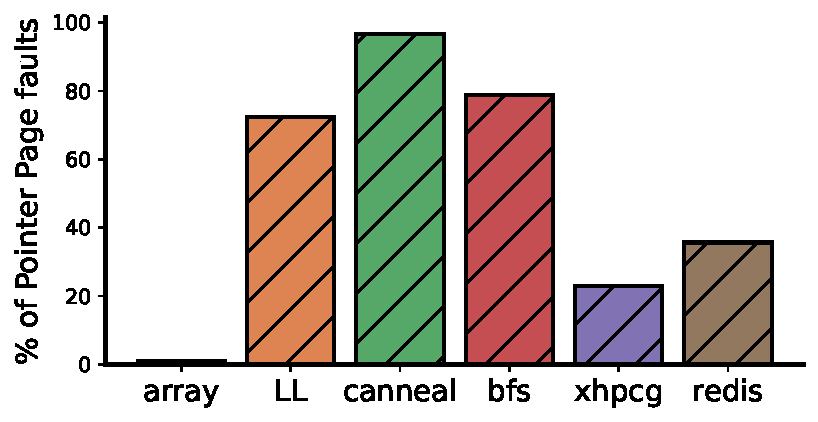
\includegraphics[height=2in]{images/bar_graph.pdf}
%        \caption{Percentage of pointer-based page faults for different workloads}
%        \label{fig:pointer_pagefaults}
%    \end{subfigure}%
%    ~ 
%    \begin{subfigure}[t]{0.7\columnwidth}
%        \centering
%        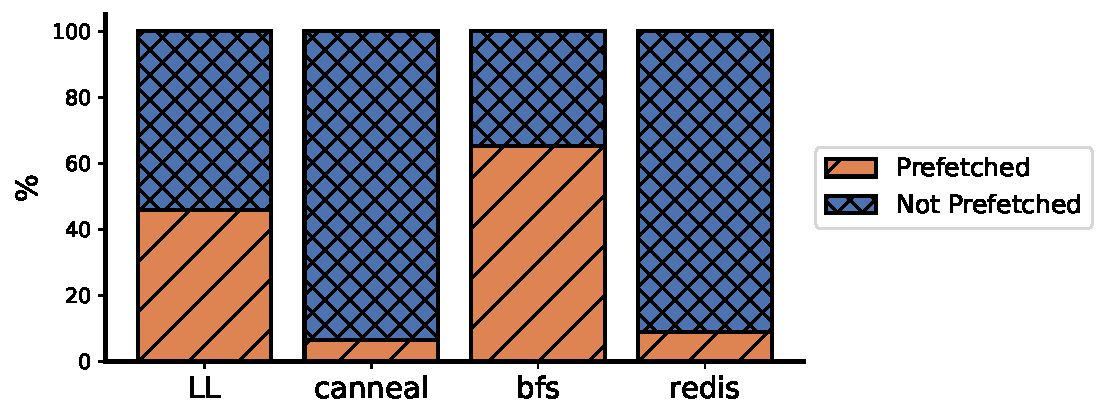
\includegraphics[height=2in]{images/divided_bar_graph.pdf}
%        \caption{Accuracy of the kernel prefetcher on pointer-based page faults.}
%        \label{fig:kernel_prefetcher_performance}
%    \end{subfigure}
    
%\end{figure*}

% To investigate which applications encounter pointer-based page faults, we developed a tool that analyzes a dynamic trace of register loads and page faults. We classify page faults into pointer-based and non-pointer-based and evaluate the performance of the default kernel prefetcher~\cite{vma-readahead}. Prior work performed a similar analysis to determine whether pointer chasing causes cache misses~\cite{cache-analysis}. However, the existence of pointer-chasing based cache misses does not guarantee the presence of pointer-based page faults. 
% For example, cache misses within a page do not cause page faults; only cache misses across pages might cause them. 
% Furthermore, page faults occur only when the application accesses swapped-out data.

% \subsection{Analyzer design} 
% Our analyzer merges two traces: a dynamic trace of all values loaded into registers and a trace of page fault addresses. A pointer is simply a memory location containing an address; without type information, it is impossible to distinguish a pointer from a non-pointer. 
% So, we borrow from prior work on cache prefetching~\cite{cache-analysis} to analyze dynamic application execution trace. If a value is loaded into a register from memory and is then used as an address or in an address computation, we consider it to be a pointer-based access. 
% For example, consider the linked list traversal and its corresponding assembly shown in \autoref{x86code}. 
% The value of \textit{curr} stored on the stack, is first loaded into register \texttt{rax} (Line 2) and subsequently accessed to load \textit{curr->next} from memory (Line 3). 
% %During the next node access, \textit{curr->next} will be accessed. 
% We classify this as a pointer-based access because the value of \textit{curr} was initially loaded into a register and subsequently used as an address. 
% If the access to \textit{curr} caused a page fault, we classify that page fault as a pointer-based page fault.

% \begin{comment}
% \begin{lstlisting}[caption={Linked list traversal example}, label={code:ll}, style=CStyle]
% struct node { ... struct node *next; }
% int main(void) {
%    ...
%    while(!curr) 
%         curr = curr->next;
%         // mov 0x2b46(%rip),%rax
%         // mov (%rax),%rax
%         // mov %rax,0x2b3c(%rip)
% }
% \end{lstlisting}
% \end{comment}

% \begin{lstlisting}[caption={x86 Assembly for traversal}, label=x86code,style=customasm,captionpos=b]
% ;curr = curr->next;
%  mov -0x600028(%rbp),%rax;load address of curr to rax
%  mov 0xff0(%rax),%rax;load the value of the curr->next
%  mov %rax,-0x600028(%rbp);store the loaded value
% \end{lstlisting}
    
% \vspace{-0.6cm}
% \subsection{Analyzer implementation}
% \begin{table}[]
% \resizebox{\columnwidth}{!}{%
% \renewcommand{\arraystretch}{1.4}
% \begin{tabular}{llc}

% \hline
% \textbf{Workload}           & \textbf{Source}    & \textbf{WSS}                 \\
% \hline
% Array streaming             & Microbenchmark    & 50\%                  \\
% Random linked list traversal (LL) & Microbenchmark    &      50\%            \\
% %Canneal                     & Parsec benchmark suite~\cite{parsec} &  50\%              \\
% %xHPCG                       & HPCG benchmark suite~\cite{hpcg}    &  50\%   \\
% Canneal                     & Parsec~\cite{parsec} &  50\%              \\
% xHPCG                       & HPCG~\cite{hpcg}    &  50\%   \\
% BFS on twitter dataset~\cite{twitter-dataset}      & GapBS~\cite{gapbs} & 25\%  \\
% %BFS on twitter dataset~\cite{twitter-dataset}      & GapBS~\cite{gapbs} (default processing system) & 25\%  \\

% Redis benchmark LRANGE      & Redis~\cite{redis} & 25\%       \\                    
% \hline
% \end{tabular}
% }

% \caption{Workloads used for analysis. 
% They represent a diverse spectrum of pointer-based fault intensity as shown in ~\autoref{fig:pointer_pagefaults}. WSS is the working set size in RAM}
% \label{tab:workloads}
% \vspace{-0.75cm}
% \end{table}

% We collect the dynamic trace of all values loaded into registers using Intel PIN (v3.26)~\cite{pin} and the page fault trace using \texttt{perf}~\cite{perf-probe} on Linux (v5.19). We run the analysis on Linux due to the availability of Intel PIN and \texttt{perf}, but we expect the analysis approach to generalize across platforms.
% We gather these traces during one program execution. We merge the two traces using timestamps and process them in sequential order. The analyzer maintains two data structures; the current state of the execution in a registers-to-value map and a set of loaded values. Once all the registers containing a particular value are overwritten, we remove the original value from the loaded values set. When a page fault occurs, the analyzer checks if the page address was loaded into a register by checking the currently loaded values set and then classifies the page fault as pointer-based if it is present. The analyzer can analyze traces in both offline and streaming mode.

% \subsection{Pointer-based page faults}
% \begin{figure}
% 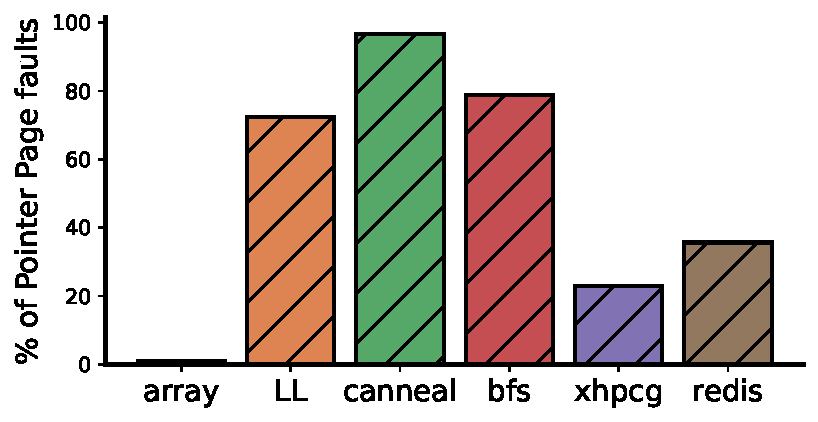
\includegraphics[height=3.3cm]{images/bar_graph.pdf}
% \caption{Percentage of pointer-based page faults for different workloads}
% \vspace{-0.25cm}
% \label{fig:pointer_pagefaults}
% %vspace{-1.3cm}
% \end{figure}

% \begin{figure}
% 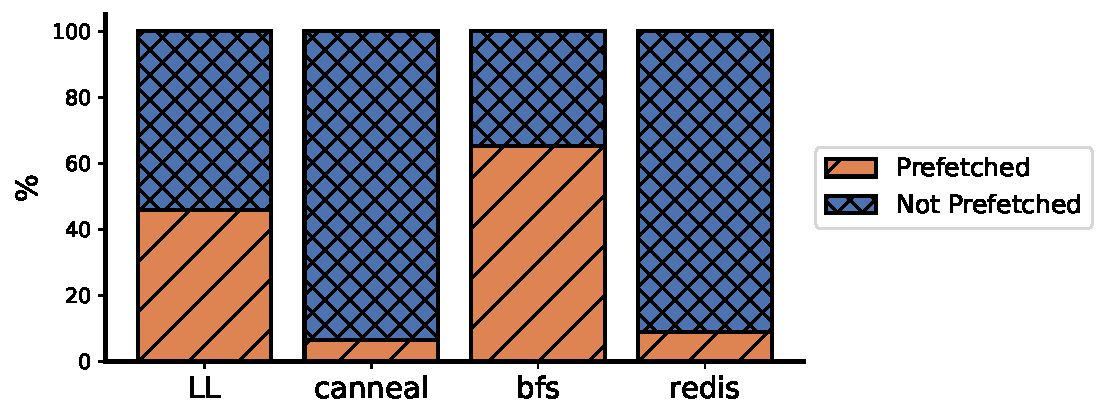
\includegraphics[height=3.3cm]{images/divided_bar_graph.pdf}
% \caption{Accuracy of the kernel prefetcher on pointer-based page faults.}
% \vspace{-0.25cm}
% \label{fig:kernel_prefetcher_performance}
% \end{figure}


% We analyzed different benchmarks (\autoref{tab:workloads}). In order to evaluate the potential of CHERI-picking in ideally suited workloads, we looked for benchmarks that demonstrate pointer-chasing behavior. We chose benchmarks based on prior work~\cite{classifying, dilos} having identified that they would benefit from pointer prefetching:
% Parsec's canneal~\cite{parsec}, xHPCG~\cite{hpcg} and Redis~\cite{redis}.
% %DiLOS~\cite{dilos} implemented an application-specific pointer prefetcher for Redis and showcased performance improvements; however, they did not analyze cache statistics. Hence, we replicated their approach. 
% To have confidence in the validity of our tool, we also designed a linked list traversal microbenchmark, which dynamically allocated page-sized nodes and ordered them randomly to render the kernel prefetcher ineffective. 
% For the array traversal microbenchmark, we allocated an array and streamed it sequentially twice. 
% To focus on page fault behavior, we constrained the program's memory using \texttt{cgroups}~\cite{cgroups}.

% \autoref{fig:pointer_pagefaults} presents our results. As we expect, a majority of the faults in the linked list microbenchmark are pointer-based, while none of the faults in the array streaming benchmark are. 
% Unsurprisingly, pointer-based page fault rates vary in other workloads, ranging from about 30\% for xHPCG 
% to almost 100\% for canneal. 
% Canneal accesses elements by indexing into two lists of pointers, so we expect it to have a majority of pointer-based faults. 
% The xHPCG benchmark maintains sparse vector objects and uses them to perform computation, leading to a lower percentage of pointer-based faults. The BFS benchmark performs breadth first search on a graph, stored in compressed sparse row format. Every access from a vertex to its children dereferences a pointer. 

% Our results suggest that some applications can benefit significantly from pointer prefetchers.
% An ideal pointer prefetcher should identify applications that can benefit from pointer prefetching without imposing overhead on applications that cannot, and achieve high prediction accuracy.



% \subsection{Performance of default kernel prefetcher on pointer-based page faults}

% The default kernel prefetchers detect sequential and strided accesses, make decisions quickly, and add little latency to the page fault path. Therefore pointer prefetchers should focus only on applications where the kernel prefetcher is ineffective. Figure \ref{fig:kernel_prefetcher_performance} illustrates the accuracy of the default kernel prefetcher~\cite{vma-readahead} on page faults that were classified as pointer-based. As expected, the results show that kernel prefetcher performance also varies, thus pointer prefetchers should be used to predict only those page faults that the default prefetcher misses. In the case of the linked list traversal, the kernel prefetcher predicts approximately 50\% of the pointer faults because the benchmark contains two loops; the first loop accesses the linked list nodes in the allocation order, while the second loop accesses them in random order. Accessing items
% in allocation order tends to produce a sequential access pattern that the default prefetcher handles well; accessing items in a random order produces an arbitrary pattern, so the default prefetcher fails. Surprisingly, although 78\% of page faults for BFS~\cite{gapbs} are classified as pointer-based, the kernel prefetcher successfully predicts 65\%, likely due to the compressed representation, which frequently places many child nodes on the same page. These applications leave limited room for improving prefetcher performance. In contrast, the kernel prefetcher predicts only about 8\% of the pointer-based faults in Redis, indicating significant potential. These findings emphasize that identifying applications where the default kernel prefetcher is ineffective is a key part of designing a pointer prefetcher.

% %Our analysis results show that important applications experience pointer-based faults and that the scope of pointer prefetchers for some applications is immense. An ideal pointer prefetcher should identify these applications without imposing a high overhead and achieve a high prediction accuracy on them.